% options:
% thesis=B bachelor's thesis
% thesis=M master's thesis
% czech thesis in Czech language
% english thesis in English language
% hidelinks remove colour boxes around hyperlinks

\documentclass[thesis=B,english]{FITthesis}[2012/10/20]

\usepackage[utf8]{inputenc} % LaTeX source encoded as UTF-8
% \usepackage[latin2]{inputenc} % LaTeX source encoded as ISO-8859-2
% \usepackage[cp1250]{inputenc} % LaTeX source encoded as Windows-1250

\usepackage{graphicx} %graphics files inclusion
% \usepackage{subfig} %subfigures
% \usepackage{amsmath} %advanced maths
% \usepackage{amssymb} %additional math symbols

\usepackage{dirtree} %directory tree visualisation

% % list of acronyms
% \usepackage[acronym,nonumberlist,toc,numberedsection=autolabel]{glossaries}
% \iflanguage{czech}{\renewcommand*{\acronymname}{Seznam pou{\v z}it{\' y}ch zkratek}}{}
% \makeglossaries

% % % % % % % % % % % % % % % % % % % % % % % % % % % % % % 
% EDIT THIS
% % % % % % % % % % % % % % % % % % % % % % % % % % % % % % 

\department{Department of software engineering}
\title{Specialized Information System Maintaining Patients Participating in Epileptosurgical Programme – Reporting Module}
\authorGN{Martin} %author's given name/names
\authorFN{Dvořáček} %author's surname
\author{Martin Dvořáček} %author's name without academic degrees
\authorWithDegrees{Martin Dvořáček} %author's name with academic degrees
\supervisor{Ing. Petr Ježdík Ph.D.}
\acknowledgements{This thesis has benefited greatly from the support of many people, some of whom I would sincerely like to thank here.

To begin with, I am deeply grateful for the support and guidance of Mr. Ježdík with whom I have a possibility to cooperate for past two years. Thanks to him, I could work on such an interesting topic as an implementation of an information system for a the biggest hospital in the Czech Republic.

Also, I owe special thanks to all my classmates that have somehow participated in the process of development of the GENEPI IS.

My sincere gratitude goes to Tim Rogers for the proofreading of my thesis.

Finally, but first in my heart, my parents and my brother are due my deep gratitude for their continued moral and financial support throughout my studies. The broad education that I was able to enjoy while growing up has proven invaluable.
}
\abstractEN{
Epilepsy is a brain disorder that affects approximately 1\% of the population. Of these, approximately 10 \% of the patients suffer from a pharmacoresistant form of epilepsy which can not be treaten by the standard medical procedures. This paper deals with the analysis, design and implementation of a reporting module to the GENEPI Information System, which was developed for the Faculty Hospital Motol by the students of FIT ČVUT, and is a key tool for the management of patients, involved in epileptosurgical programme. Currently in the epileptosurgical programme are involved 150 patients, mostly children, and its beginning dates back to 2000. GENEPI IS, and thus the reporting module, is software that was developed from the beginning according to the specific requirements of doctors who use it. Given that it stores unique information, which also may contain sensitive information, the resultant product was developed under special claims. Among those included robustness, reliability and safety aspects.
}
\abstractCS{Epilepsie je onemocnění mozku, které postihuje přibližně 1\% populace. Z toho přibližně 10\% pacientů trpí farmakorezistentní formou epilepsie, při které se nedají použít standardní léčebné postupy. Tato práce se zabývá analýzou, designem a implementací reportovacího modulu do Informačního Systému GENEPI, který byl vyvíjen na zakázku pro Fakultní Nemocnici Motol studenty FIT ČVUT, a který je klíčovým nástrojem pro správu těchto pacientů zapojených do epilepticko-chirurgického programu. V současné době je do epilepticko-chirurgického programu zapojeno na 150, převážně dětských, pacientů a jeho začátek se datuje do roku 2000. GENEPI IS, a tím pádem i reportovací modul, je software, který byl od začátku vyvíjen na základě specifických požadavků lékařů, kteří jej používají. Vzhledem k tomu, že uchovává unikátní data, která zároveň mohou obsahovat citlivé údaje, tak byly na výsledný produkt při vývoji kladeny zvlášní nároky. Mezi ty patřila robustnost, spolehlivost a především bezpečnost. 
}
\placeForDeclarationOfAuthenticity{Prague}
\keywordsCS
{
export dat, přístup na základě uživatelských rolí, anonymizace dat, reportovací modul
}
\keywordsEN
{
export of data, access acording to the user roles, data anonymization, reporting module
}
\declarationOfAuthenticityOption{1} %select as appropriate, according to the desired license


\begin{document}

% \newacronym{CVUT}{{\v C}VUT}{{\v C}esk{\' e} vysok{\' e} u{\v c}en{\' i} technick{\' e} v Praze}
% \newacronym{FIT}{FIT}{Fakulta informa{\v c}n{\' i}ch technologi{\' i}}

\chapter{Introduction}
The reporting module, as part of the GENEPI - information system, adds an important functionality to this software. Thanks to this module the user will be able to export data saved in the system to sundry formats. This is useful for the doctors that take care of patients with epilepsy, as well as for the researchers that make analysis above the data from this system. The goal was to extend the IS with additional functionality without letting the user notice he's even using further extension. Therefore the reporting module was delicately worked into the existing source code of the GENEPI IS, using the same design patterns and approaches as the rest of the IS.

The GENEPI IS should replace the original information system that was used in the Faculty Hospital Motol in Prague for maintaining patients in its epileptosurgical programme. The main reasons for replacing the original information system was the fact that it didn't comply with the current requirements of the doctors, contained bugs and its design wasn't optimal. Because of the uniqueness of stored data and because of the special requirements of the system itself, there was no free software available that would be suitable and thus it was needed to create custom information system.

I chose to participate in this project, although I knew it would not be easy. The main reasons that led to selection of participation in the development of the GENEPI IS were the facts that it is a software that will be deployed in the production environment to be used by real users and can help to improve the state of health of real people. 

In the following chapters the reader will become familiar with the GENEPI IS, the process of analysis, design and realisation of the reporting module, as well as with the process of testing and will see a few examples of exports done by the reporting module.

\chapter{Current status}

That the reader can fully understand the functioning of the reporting module, first of all it is needed to introduce the information system that it extends. The GENEPI information system was being created within the subjects BI-SP1 and BI-SP2 at the Czech Technical University, Faculty of Information Technologies in the school year 2012/2013 as a student project. You will find these projects on enclosed CD.

GENEPI IS is being developed in the java programming language, using frameworks\footnote{An abstraction in which software providing generic functionality can be changed by code additionally added by a programmer}  Spring 4.0.2 and Hibernate 4.3.4. The front end part is realized via JSP, using HTLM5, JavaScript and CSS. Libraries that were used to ease the programming of the front end were Twitter Bootstrap 3.3.1 and jQuery 2.1.0.  MySQL 5.5 was chosen as a database and  Apache Tomcat 7 as an application server. All of the used software and libraries are distributed under some kind of free license. GENEPI IS is a bilingual software due to the expected deployment in the Miami Children's hospital in Florida, the United States of America. Languages that are currently supported, are Czech and English, nevertheless thanks to the suitably implemented localization it is easy to extend the application to add any other language. During the whole period of the programming of the system, the team consulted the approach often  and regularly with the contracting authority, to fully meet the needs of the doctors.

\section{Functional Requirements}
A functional requirement defines a set of inputs, the behavior, and outputs of a system or its components. Functional requirements may include data manipulation and processing, data validation as well as implemented features such as searching, export, etc.
\begin{itemize}
  \item Patient files
  \item Medical history records of patients
  \item Advanced Search according to given parameters
  \item Export of the records to sundry formats
  \item Verification of patients
  \item Managing users and roles
  \item Quicksearch in patients card index
  \item Validation of patients
  \item Versioning of database changes
  \item Hiding patients and their medical records instead of deleting
\end{itemize}

\section{Non-functional Requirements}
A non-functional requirement is a requirement that specifies criteria that can be used to judge the the system. Usually those are security, accessibility or reliability.
\begin{itemize}
  \item Role-based access control
  \item Robustness
  \item Reliability
  \item Solution based on free technologies
  \item Security
  \item Responsive design\footnote{Design that provides optimal viewing experience on any kind of device} 
\end{itemize}


\section{Used back end technologies}
\begin{enumerate}

\item{Java 7}

Java is the foundation for virtually every type of networked application and is the global standard for developing and delivering embedded and mobile applications, games, Web-based content, and enterprise software. Java is designed to enable development of portable, high-performance applications for the widest range of computing platforms possible. By making applications available across heterogeneous environments, businesses can provide more services and boost end-user productivity, communication, and collaboration—and dramatically reduce the cost of ownership of both enterprise and consumer applications.\cite{java}

\item{Apache Tomcat application server}

Apache Tomcat is an open source software implementation of the Java Servlet and JavaServer Pages technologies. Apache Tomcat is developed in an open and participatory environment and released under the Apache License version 2. Apache Tomcat powers numerous large-scale, mission-critical web applications across a diverse range of industries and organizations.\cite{apache}

\item{MySQL Community Server}

The MySQL software delivers a very fast, multi-threaded, multi-user, and robust SQL database server. MySQL Server is intended for mission-critical, heavy-load production systems as well as for embedding into mass-deployed software.\cite{mysql}

\item{Spring Framework}

The Spring Framework provides a comprehensive programming and configuration model for modern Java-based enterprise applications - on any kind of deployment platform. A key element of Spring is infrastructural support at the application level: Spring focuses on the "plumbing" of enterprise applications so that teams can focus on application-level business logic, without unnecessary ties to specific deployment environments.\cite{spring}

\item{Spring MVC}

Spring's Web MVC framework is designed around a DispatcherServlet that dispatches requests to handlers, with configurable handler mappings, view resolution, locale and theme resolution as well as support for upload files. \cite{springmvc}

\begin{figure}
	\centering
 	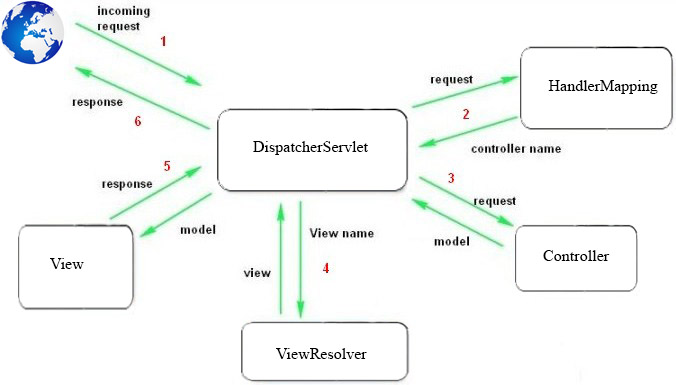
\includegraphics[width=1\textwidth]{images/SpringMVC.jpg}
 	\caption{Spring MVC web-flow}
 	\label{fig:springMVCWebFlow}
\end{figure}


\item{Spring Security}

Spring Security is a powerful and highly customizable authentication and access-control framework. It is the de-facto standard for securing Spring-based applications.\cite{springsecurity}


\begin{figure}
	\centering
 	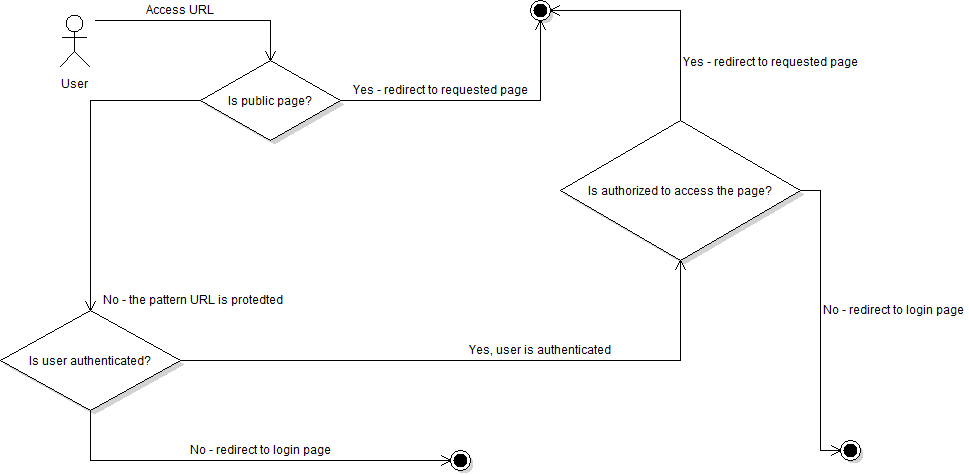
\includegraphics[width=1\textwidth]{images/SpringSecurity.png}
 	\caption{Authentication and Authorization flow}
 	\label{fig:springSecurity}
\end{figure}



\item{Hibernate}

Hibernate takes care of the mapping from Java classes to database tables, and from Java data types to SQL data types. In addition, it provides data query and retrieval facilities. It can significantly reduce development time otherwise spent with manual data handling in SQL and JDBC. However, unlike many other persistence solutions, Hibernate does not hide the power of SQL from you and guarantees that your investment in relational technology and knowledge is as valid as always.\cite{hibernate}

\end{enumerate}


\section{Used front end technologies}
\begin{enumerate}

\item{HTML5}

HTML5 contains powerful capabilities for Web-based applications with more powerful interaction, video support, graphics, more styling effects, and a full set of APIs\footnote{A set of functions, classes or protocols of a library that can be used by a programmer}. HTML5 adapts to any device, whether desktop, mobile, tablet or television.\cite{html}

\item{JavaScript}

JavaScript (often shortened to JS) is a lightweight, interpreted, object-oriented language with first-class functions, most known as the scripting language for Web pages, but used in many non-browser environments as well such as node.js or Apache CouchDB. It is a prototype-based, multi-paradigm scripting language that is dynamic, and supports object-oriented, imperative, and functional programming styles.\cite{javascript}

\item{CSS}

Cascading Style Sheets (CSS) is a simple mechanism for adding style (e.g., fonts, colors, spacing) to Web documents.\cite{css}

\item{JSP}

JavaServer Pages (JSP) technology enables Web developers and designers to rapidly develop and easily maintain, information-rich, dynamic Web pages that leverage existing business systems. As part of the Java technology family, JSP technology enables rapid development of Web-based applications that are platform independent. JSP technology separates the user interface from content generation, enabling designers to change the overall page layout without altering the underlying dynamic content.\cite{jsp}

\item{Twitter Bootstrap}

Twitter Bootstrap is the most popular front-end framework for developing responsive, mobile first projects on the web. \cite{bootstrap}. It is built with HTML, CSS and JavaScript. Thanks to this framework it was much easier to create a responsive front end with a pleasant and ergonomic look and feel.

\item{jQuery}

jQuery is a fast, small, and feature-rich JavaScript library. It makes things like HTML document traversal and manipulation, event handling, animation, and Ajax much simpler with an easy-to-use API that works across a multitude of browsers. With a combination of versatility and extensibility, jQuery has changed the way that millions of people write JavaScript.\cite{jQuery}

\end{enumerate}


\chapter{Goals}

The goal of my bachelor's thesis was to create the reporting module for the GENEPI IS, that would meet the requirements of the health care professionals and researchers that will use it.

Since the GENEPI IS is accessed by various types of users, it was needed to adapt the reporting module to this fact. One of the requests to meet this end was that the data has to be able to be exported to more formats. Specifically, the formats pdf, docx, xls, csv and txt.

Also among the important requirements included was that it has to be able to modify the scope of the exported data based on user needs, save and load export configurations, automatic and optional data anonymization and user-friendly interface.

Of course there has to also be data security to prevent access to sensitive patient data to users without proper permission.

The main goals consequently were:
\begin{itemize}
  	\item Implement export to pdf, docx, xls, csv and txt format
  	\item Implement export configuration
  	\item Allow the user to save and load customized configuration
 	\item Allow the user to anonymize exported data 
 	\item Anonymize exported data automatically if the user doesn't have sufficient privileges
\end{itemize}

\chapter{Analysis and design}
The reporting module, as well as the whole information system, was designed given the requested robustness, accessibility, reliability and the cleanness of the source code. GENEPI IS has a three-tier architecture driven by a Spring MVC module, uses access according to the roles of the users via Spring Security module and thanks to the optimalized data layer using the Hibernate framework, it saves the computing resources and facilitates developers to understand and extend the source code.

Due to the fact that users who will work with the exported data have different levels of access and different requirements on the format of the exported data there was a need to make the module able to anonymize sensitive data as well as to export data to different formats. The contracting authority also requested that the user could choose which data he would want to export.

\section{Design of the reporting module}
Architecture of the reporting module doesn't differ from the architecture of the rest of the information system. Thanks to this I was able to guarantee the robustness and the security of this module. It has also provided me an easy and elegant way to access the other components in the system.

In this tree diagram you can see the parts of the IS that concern the reporting module:

	\dirtree{%
		.1 Backend.
		.2 src.
		.3 main.
		.4 java\DTcomment{java classes}.
		.5 cz.
		.6 cvut.
		.7 fit.
		.8 GENEPI.
		.9 businessLayer.
		.10 service\DTcomment{interface of the services}.
		.10 serviceImpl\DTcomment{implementation of services}.
		.10 BO\DTcomment{Business Objects}.
		.9 dataLayer.
		.10 DAO\DTcomment{interface of the DAO}.
		.10 DAOImpl\DTcomment{implementation of DAO}.
		.10 entity\DTcomment{entities}.		
		.9 presentationLayer\DTcomment{controllers}.
		.4 resources\DTcomment{property files}.
		.4 webapp\DTcomment{files for front-end}.
		.5 resources\DTcomment{front-end libraries, pictures and other media}.
		.5 WEB-INF.
		.6 tags\DTcomment{templates for jsp}.
		.6 views\DTcomment{jsp files}.
	}


\subsection{Design of the back end part}
The back end part of the reporting module was designed to follow the three-tier architecture of the rest of the system. Thus the classes that this module uses, are devided into three different packages. Every package contains classes that belong to the same tier. These packages are called Presentation layer, Business layer and Data layer. 

\subsubsection{Presentation layer}
In the presentation layer there is a controller - a Spring MVC component that calls up a function according to the HTML request and its URL that is mapped to a particular function. This function executes simple operations such as verification of passed parameters and calls to the other layers. The results of the functions from the other layers may be saved to a org.springframework.ui.Model object and passed to the front end. This layer never executes more complicated actions as those should be done within the Business layer, nor does access the database as this should be done within the Data layer. The functions of a controller usually return the name of a view - a .jsp file - that should be displayed to a user.
\subsubsection{Business layer}
There are three packages in in this tier - concretely these are service, serviceImpl and BO. 

Service contains interfaces whereas serviceImpl contains classes that implement those interfaces from the service package. It is analogical as in the Data tier which I will describe in greater detail in the next paragraph.

In serviceImpl classes there is usually implemented some more complicated logic that shouldn't be implemented within the Presentation layer, like adjusting of BOs, sorting of lists of objects under some conditions as well as many other actions.

The third package - BO - contains classes that transform the classes from the form in which the data come from the database - in the entity classes - to a form that is more appropriate for work within the Business tier.
\subsubsection{Data layer}
This layer contains three packages - DAO, DAOImpl and entity. In the DAO package there are interfaces of the data access objects, in DAOImpl are the classes that implement the interfaces from the DAO package and finally in the entity packag, we can find the entity classes.

In DAOImpl classes you find the functions that are used to access the database and to get some data from it. There is a direct use of hibernate functions or queries in HQL.

In the entity classes is described how the structures of the tables in the database look. Every entity contains a property for every single column of the table. The type of this variable must match the type of the column of the table. If these conditions aren't satisfied the database query will fail and the AS will throw out org.hibernate.MappingException.

Every property has to have a getter and a setter as well. Thanks to anotations from javax.* and org.hibernate.validator.constrains.* it is possible to check the requirements for attributes of the input that should be saved to the database, i.e., minimal or maximal size, regexp pattern or if the input is blank or NULL.

A Hibernate annotation, @Column, is also mandatory as it describes the mapping of the property to the particular table in the database.

I would like to point out the generic GenericDAO and GenericDAOImpl classes that have been implemented.
These are abstract classes that were implemented to ease the process of programming of the other DAO and DAOImpl classes.

In the GenericDAOImpl class there are implemented the most used methods that may be used by any service such as save, delete, getCount, getCountOfUnhidden, findByID and many other. The GenericDAO class is an interface of the GenericDAOImpl class as is usual in the rest of the project. 

The other DAO and DAOImpl methods extend these generic classes so that it wasn't subsequently needed to implement these basic functions to every single class and the programmer had to programme only those functions that were unique for that particular class.

\subsection{Design of the front end part}
As well as the back end part, the front end had to follow the style and design of the rest of the system. If I haden't done so, the work with the reporting module could be confusing for users. On the basis of these facts, it was needed to implement a front end based on the same technologies as the rest of the GENEPI IS. Thanks to this approach the User Experience\footnote{User's behaviors, attitudes, and emotions about using a system or service} from work with this module is positive and the user accepts the reporting module as an integral part of the IS.

\chapter{Realisation}
In this chapter, I would like to describe how the export, its customization and security was implemented. I would also like to describe the inner logic used while performing these actions. In the end, it is also needed to familiarize the reader with the form of the front end and describe its sections individually.

The standard approach when performing an export is as follow:
\begin{enumerate}
\item{ The user chooses in the export view the properties that he wants to include in the exported file, the format, anonymization option and hits the export button }
\item{ The PatientExportPOST method in the PatientController class is called up and according to the given parameters it calls up the method to export the data to the right format. It also checks if the data should be anonymized and if the user isn't authorized to see sensitive data then it sets the anonymize flag to true automatically. All given parameters with all of this information are passed to the called upon export function in the Bussines tier.}
\item{ In this step we've moved from the Presentation tier to the Business tier, where the methods from the Data layer are called to get pateint data. Then one of the methods for export to a particular format is called. This is the part where the data is being written to the file itself. The program iterates through all the patients that the user wanted to export and gradually prints out their data.}
First the patient's header is printed out. This header contains information about the patient such as his age, gender, age at the onset of epilepsy and other important data. It may also contain sensitive data such as his name, address or other contact information.
\item{ In the last step the user is redirected to an URL of the newly created file with exported data to download. This file persists on the server and can be repeatedly downloaded. The time that this file is accessable depends on the setting of the server CRON\footnote{A time-based job scheduler in Unix-like operating systems.}, as this should regulary delete old files in the directory dedicated for export files.}

\end{enumerate}

\begin{figure}
	\centering
 	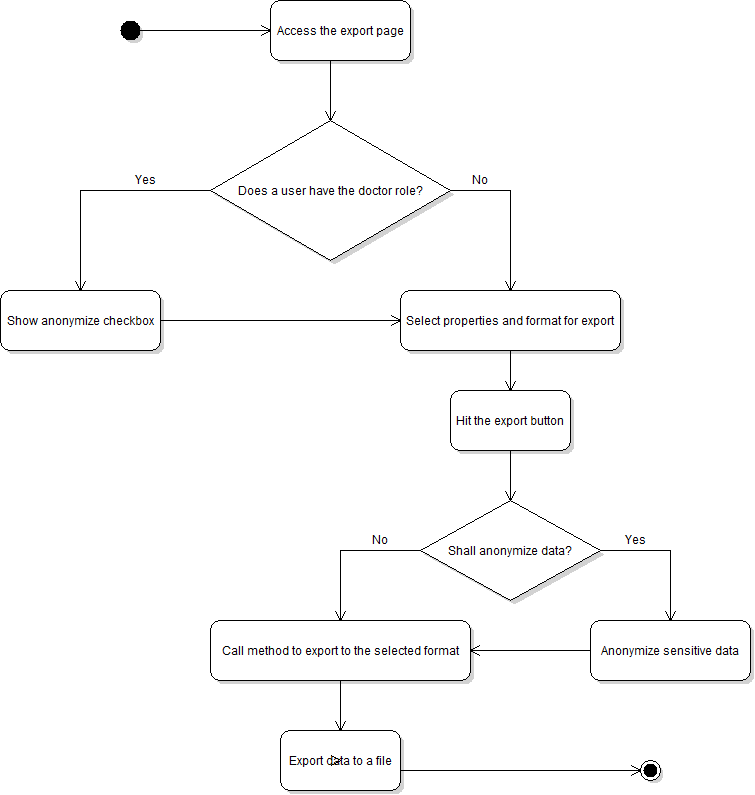
\includegraphics[width=1\textwidth]{images/exportDiagram.png}
 	\caption{Export activity diagram}
 	\label{fig:exportDiagram}
\end{figure}

The goal was to make the whole process secure, reliable and easy to understand for any programmer reading the code, as well as for the user accessing the reporting module. Thanks to the chosen design and implementation approach these requirements were satisfied.
\section{Customization of the export}
There was a strong demand from the contracting authority to create a module that would let the user customize the report. Every patient can have fifteen cards filled in. This means arround 340 properties that can be stored for every single patient. Nevertheless not all of them are needed to be exported in certain situations. Therefore it was necessary to implement some solution that would allow a user to select only those cards or properties of those cards that should be exported.

Due to the high amount of those properties, it was quite challenging to create a solution that would meet the requirements and will be user-friendly at the same time. I've chosen a treeview on the front end and a special entity on the back end.

On the front end there was implemented a customized treeview, where every item has a checkbox. Patient's cards are represented by the nodes, whereas porperties of these cards can be represented by the leaves of this tree or nodes as well. They may be nodes if they denote some category that can hold some properties that couldn't exist without their parent category. By checking and unchecking these items, the user can choose, what all should be involved in the exported data. When unchecking the node all leaves of this node are aslo deselected. On the other hand, by selecting even a single leaf from an unselected branch, the parent node is selected as well.
Here I attach a simple example of the treeview I was writing about:


	\dirtree{%
		.1 Anamnesis\DTcomment{anamnesis card}.
		.2 Anamnesis property.
		.2 Another anamnesis property.
		.1 Seizures\DTcomment{seizure card}.
		.2 Seizure property.
		.2 Another seizure property.
		.1 ....
		.1 ....
		.1 Neuropsychology\DTcomment{neuropsychology card}.
		.2 Neuropsychology inner node.
		.3 Neuropsychology property.
		.3 Another Neuropsychology property.
		.2 Another Neuropsycholgy inner node.
		.3 Neuropsychology property.
		.2 Neuropsychology property.
		.1 ....
		.1 ....
		.1 Outcome\DTcomment{outcome card}.
	}

After confirming the export form, the state of the treeview is saved to an instance of an entity called ExportParams. This entity has a boolean property for every single value from the treeview in the export form. Thanks to this I am able to determine which properties the user wanted to export and which he didn't. It gives me another advantage - I can save the current setting of the treeview for a later usage, but I will write about this feature later.

\section{Export to the particular formats}
During the  programming of the classes that procure the logic of the reporting, I was trying to use the fact that there already exist java libraries that can export data to docx, pdf, xls and csv formats. I also avoided the duplication of the code by transforming data from one format to another. Thanks to these measures, it is much easier to make changes in the code of the classes that handle export itself and it also eases the understanding of the code for anybody reading it.
\subsection{txt}
Export to the text format is realized by components from java.io.* package. Specifically java.io.FileOutputStream, java.io.OutputStreamWriter and finally java.io.BufferedWriter. Output is encoded to the UTF-8 format. Every property is printed out to a new line, sections are delimited by dash lines, star lines or empty lines.
\subsection{docx}
Export to the docx format was not as easy as to the txt, so I decided to look up suitable libraries, compare them and use the one that would best suit my needs. After researching the possible solutions I ended up with two libraries - Apache POI and docx4j.

I've chosen to use docx4j because it provided me more functionalities and clearer API then Apachi POI could. The main problem I had with Apachi POI was the formating of the cells when I wanted to format data to the tables. I could hardly adjust the size of the cells and redefine my own styles of headers and text. Docx4j provided me a really easy and elegant way to solve these issues.
\subsection{xls}
As well as for the docx format, I used the fact that there already were programmed libraries for export to xls.
I've chosen to use Apache POI library, as this library provides me eveything I need to export data to an xls file, such as merged cells, creation of new lists and changing the background color of the cells.
\subsection{pdf}
There are of course java libraries that provide you some way to export data to pdf format as well, nevertheless I've chosen a different approach. While I already had implemented the export to docx, I've chosen not to implement export to pdf, but instead to create a file with data exported to docx and using the classes from apache.poi.xwpf.converter.* package to convert this file to pdf. Thanks to this approach I didn't duplicate the code because the only logic needed to format and print out the data for export was already implemented in the export to docx. After transforming docx file to pdf, the original docx file is deleted and only the newly created pdf file persists.
\subsection{csv}
Before I started to implement the export to csv format, I was also thinking whether I should implement the whole logic of export to csv, but decided to proceed similarly as in the case of implementation of the export to pdf. Nevertheless, in this case I don't use a file with data exported to docx, but a file created by export to xls, as this format can be easily transformed to csv and vice versa. During the export to csv I create at first an xls file with exported data and then walk through this file and print out the values to the file via the classes from java.io.* package. These are the same classes that have been used in the export to txt. Based on the requirements of the contracting authority commas, as a standard delimiter in csv format, has been replaced with semicolons. The main reason of this change was the fact that every card that a patient may have contains a comment field, which is  text and which may contain commas. As the semicolon is a much less used character in sentences, it was decided to use it as a delimiter. Otherwise the report could look confusing for the user.
\section{Security and anonymization}
In GENEPI IS there are 5 main levels of access, according to the visibility of the patient's data.

	\begin{enumerate}
	\item{Users}
	
	The User role is a basic role that every new user gets from the system by default. This role allows you to acces the homepage 	and your user profile. Without any further role, the user is not allowed to perform any further actions.

	\item{Administrators}

	Administrators don't have any access to the patient's data. They are not even able to access the URL to view or export this data. They're the only users who may create new users and edit users' roles. They may also edit a users' details and change passwords.
	\item{Researchers}

	Researchers have limited access to patients' data - they are not allowed to see sensitive data. Nevertheless they are still able to see lists of users, with limited options to use advanced search and export anonymized data. Researchers are not allowed to modify patients' data.
	\item{Doctors}

	Doctors have full access to patients' data, they are allowed to add new patients and modify their data. Nevertheless, after every change the patient is set as unverified. This means that those changes weren't checked by an authorized person, can't be with certainty trusted and shouldn't be included in any research. Doctors by default don't have authority to verify patients whose data were changed and are set as unverified.

	\item{Superdoctors}

	Users with the role of Superdoctor have the same priviledges as users with the role of Doctor. Moreover they have the right to verify unverified patients.

	\end{enumerate}

Because of this fact it was needed to implement some way to anonymize the exported data. To the reporting module I implemented two types of anonymization - optional and manadatory.

Optional anonymization is accessable to doctors and superdoctors only. Before they perform the export, they can decide if they want to anonymize the exported data. This could be useful, for example, in situations where the doctor needs to provide the data to somebody who normally doesn't have access to the system and at the same time shouldn't see the sensitive informations. On the other hand the doctor still has the possibility to export unanonymized data, which might be useful for medical purposes.

Mandatory anonymization is done automatically, when somebody who doesn't have a sufficient access level wants to export data. This feature will prevent anybody who is unauthorized from seeing the sensitive data of the patients. Anonymized data will be mostly used by researchers who make analysis upon the data and don't need to know the names and addresses of patients because they can distinguish them according to their IDs, which is a mandatory property  printed out for every patient in every export.
\section{Custom configurations}
Customization of the configuration of exported data was one of the key features of this module. Due to the fact that there are several types of users who work with this IS it's necessary to take account of how the ways they need to use it differs. Researchers usually do some analysis above some part of the data from the IS, whereas doctors usually need some more complex report about a patient's state of health and the treatment process.

It is obvious, that setting these configurations will be required regulary, as it is not expected that users would need to create a unique configuration for every single export he'd like to perform. Because of this, it was decided that users should have an option to save their adjusted configuration for a later use. The reporting module for GENEPI IS distinguishes two types of saved configurations.

The first is the configuration saved by a user with the Superdoctor role. This configuration may be set as generic. That means that the user chose to allow his configuration to propagate through the system so other users may see and use it.

The other type is the user's private configurations. Every user with a sufficient access level to access the export view is allowed to create and use them. These are configurations that were created by a user himself and are available only to him. The other users are not able to use these configurations, nor to see them.

Deletion of configurations is possible as well. Private configurations can be deleted by a user who can see them in his list of private configurations and not by anybody else. 

On the other hand generic configurations are visible to all users in the system, therefore it is necessary to determine if a user who wants to delete some generic configuration has even the right to perform this action. To delete a generic configuration the user has to own a Superdoctor role. Then he's allowed to delete any generic configuration created by any other user. If the user doesn't have a Superdoctor role, then the delete button for generic configurations is not even displayed to this user in the export view.
In the following pictures you can see the activity diagram of saving and then deleting of a configuration from the point of view of the user.

\begin{figure}
	\centering
 	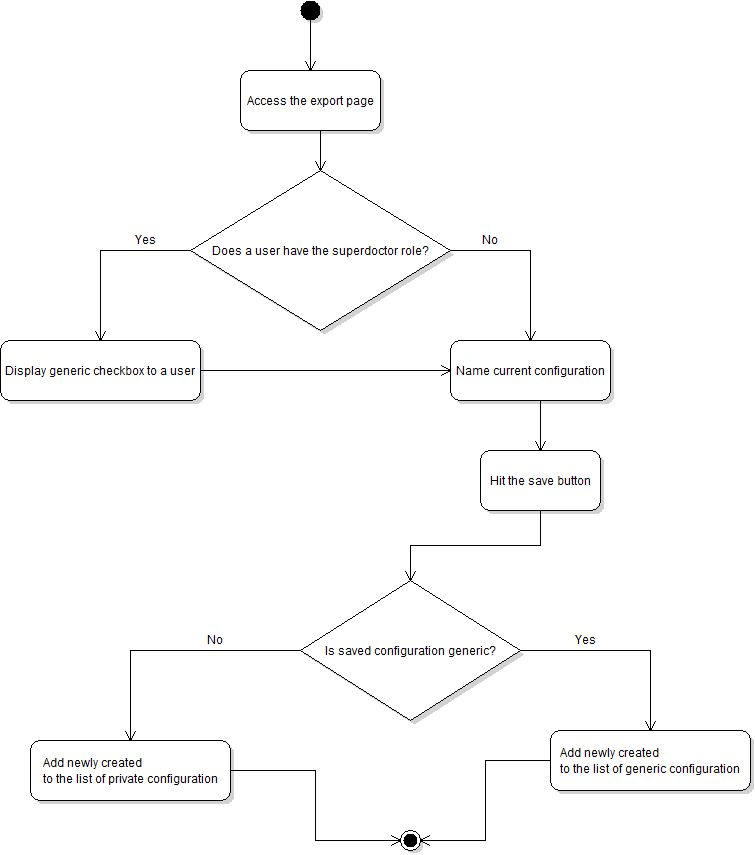
\includegraphics[width=1\textwidth]{images/createConfigurationDiagram.png}
 	\caption{Create configuration activity diagram}
 	\label{fig:createConfigurationDiagram}
\end{figure}

\begin{figure}
	\centering
 	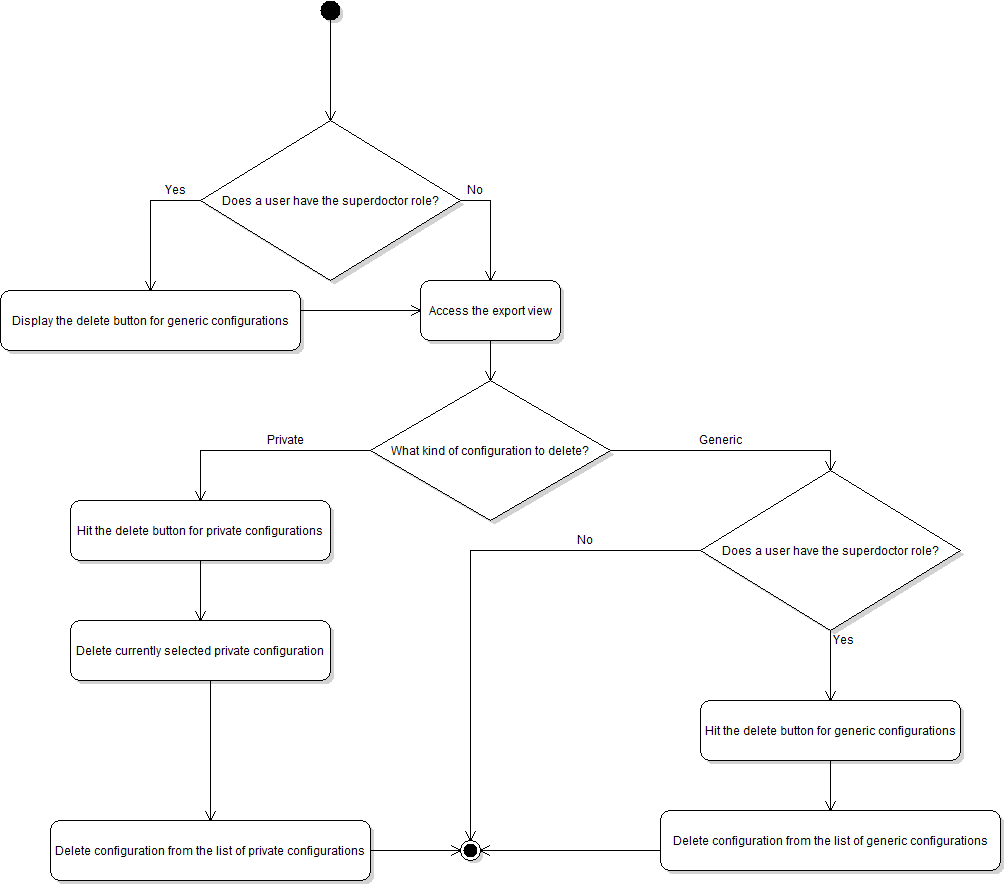
\includegraphics[width=1\textwidth]{images/deleteConfigurationDiagram.png}
 	\caption{Delete configuration activity diagram}
 	\label{fig:deleteConfigurationDiagram}
\end{figure}


\section{Graphical user interface of the reporting module}
In the following pictures I'll explain all the components used to control the export view. During the phase of design and implementation of the view I had to take into account the fact that users of this module need a user-friendly interface that would provide them all of the tools necessary customize exports.

In the first picture, you can see the interface for loading and deleting custom configurations. In the first row there is a combobox with generic custom configurations which the user may load or even delete, if he's the creator of this configuration.

\begin{figure}
	\centering
 	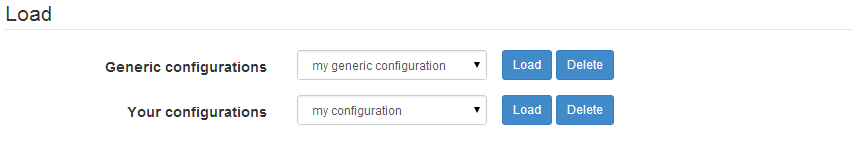
\includegraphics[width=1\textwidth]{images/load.png}
 	\caption{Loading and deleting of a custom configuration}
 	\label{fig:load}
\end{figure}


In the next picture there is displayed a section for export itself. First a list of IDs of the patients that are prepared for an export. The user may access the patient's overview by clicking his ID. Next it's necessary to choose the format for export via several radiobuttons. In the case that the user chooses as a format docx or pdf, a checkbox appears and allows him to choose if exported data should be formated into tables or as a text. If the user has a Doctor or Superdoctor role assigned, then he's able to see a combobox that allows him to anonymize exported data.

\begin{figure}
	\centering
 	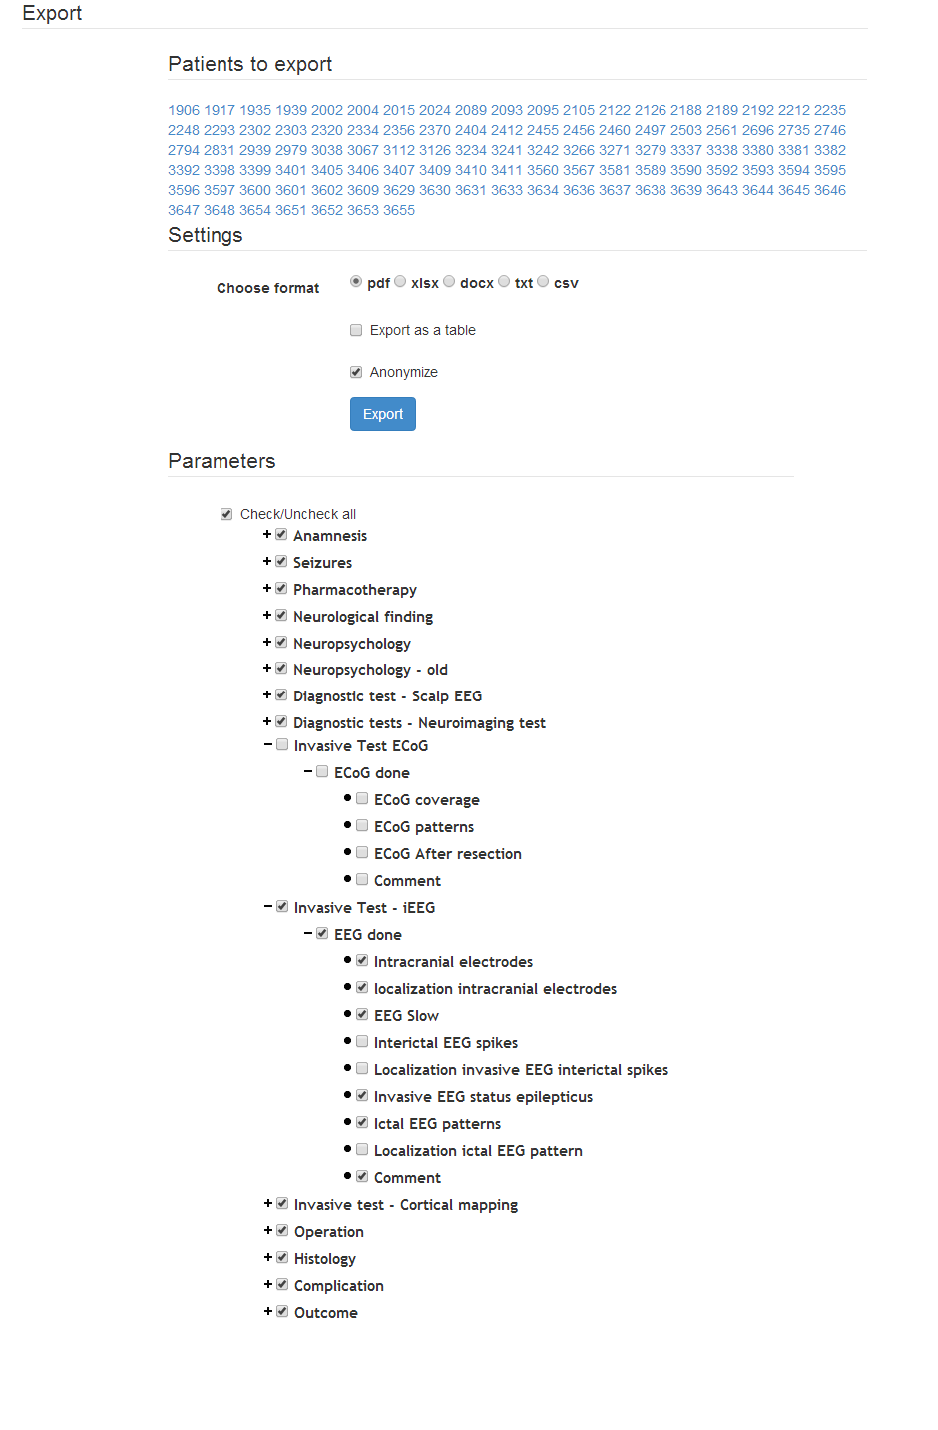
\includegraphics[width=1\textwidth]{images/export.png}
 	\caption{Selection of format and customization of an export}
 	\label{fig:export}
\end{figure}


In the last picture you can see the interface for saving custom configurations. There is a textfield for naming the configuration and if the user has a Superdoctor role, then he may check the checkbox to make it generic.

\begin{figure}
	\centering
 	
\includegraphics[width=1\textwidth]{images/save.png}
 	\caption{Saving a custom configuration}
 	\label{fig:save}
\end{figure}


\chapter{Testing and Examples}

Testing of the reporting module as well as the GENEPI IS itself was performed during the development by the developers themselves and by a member of the team who held the position of a tester. After key  functionalities were implemented, Ing. Ježdík Ph.D obtained access to the system and tested it with normal use cases. He of course had many requests for changes that would improve the application or found bugs that requiered fixing. Currently the GENEPI IS with reporting module should be deployed on produciton servers in the Faculty Hospital Motol and will fully replace the existing application. As in most of the cases from the commercial sector, it is expected, that users will also make some requests for changes. But those are expected to be minor change requests, mostly on the front end and should be implemented within a few MD.

In the following screenshots the reader can see a few examples of how the export files created by the reporting module look. I also enclose a simple example of an analysis made on the basis of data from GENEPI IS, that were exported into xls. All these examples spring from real data, currently saved in the IS, but they were anonymized of course. You may find these files enclosed on the CD as well.

\begin{figure}
	\centering
 	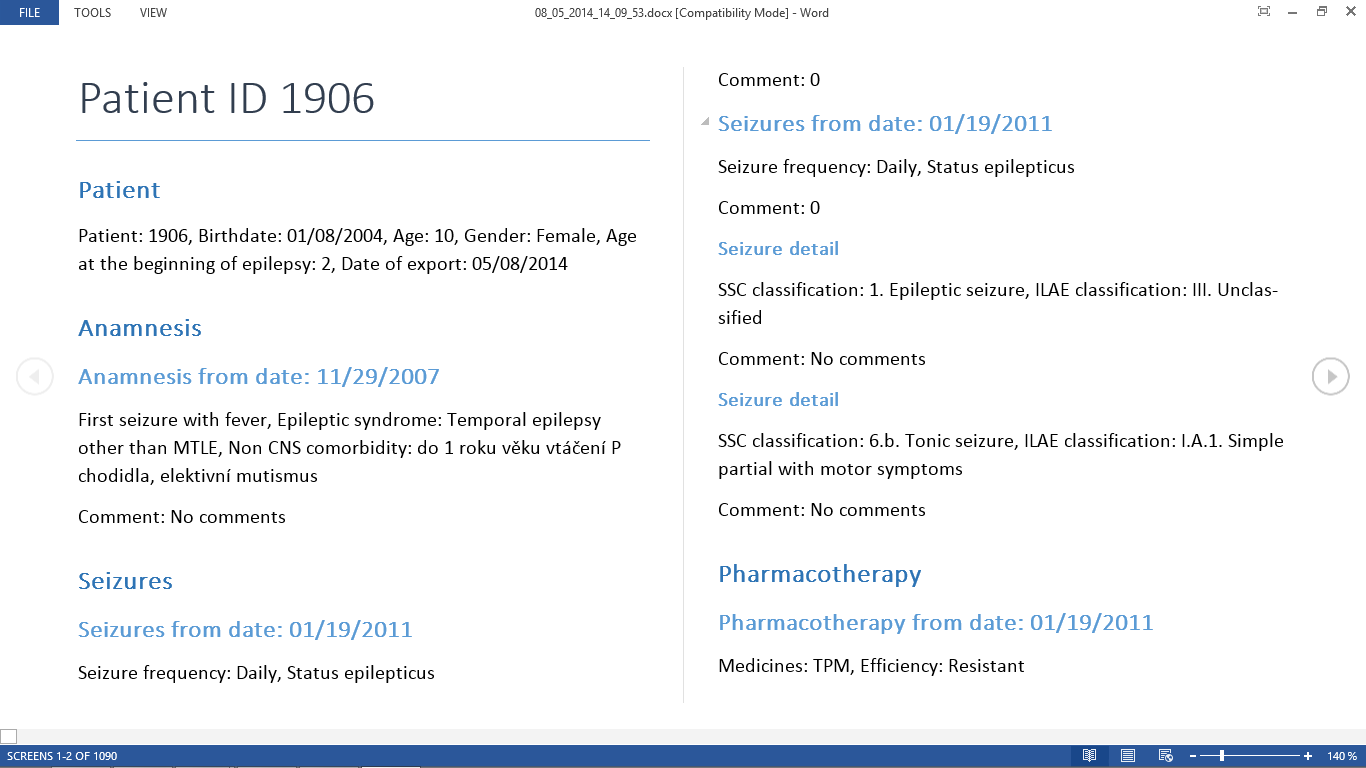
\includegraphics[width=1\textwidth]{images/docxExport_1.png}
 	\caption{Screenshot of an export of all patients to docx}
 	\label{fig:docxExport_1}
\end{figure}

\begin{figure}
	\centering
 	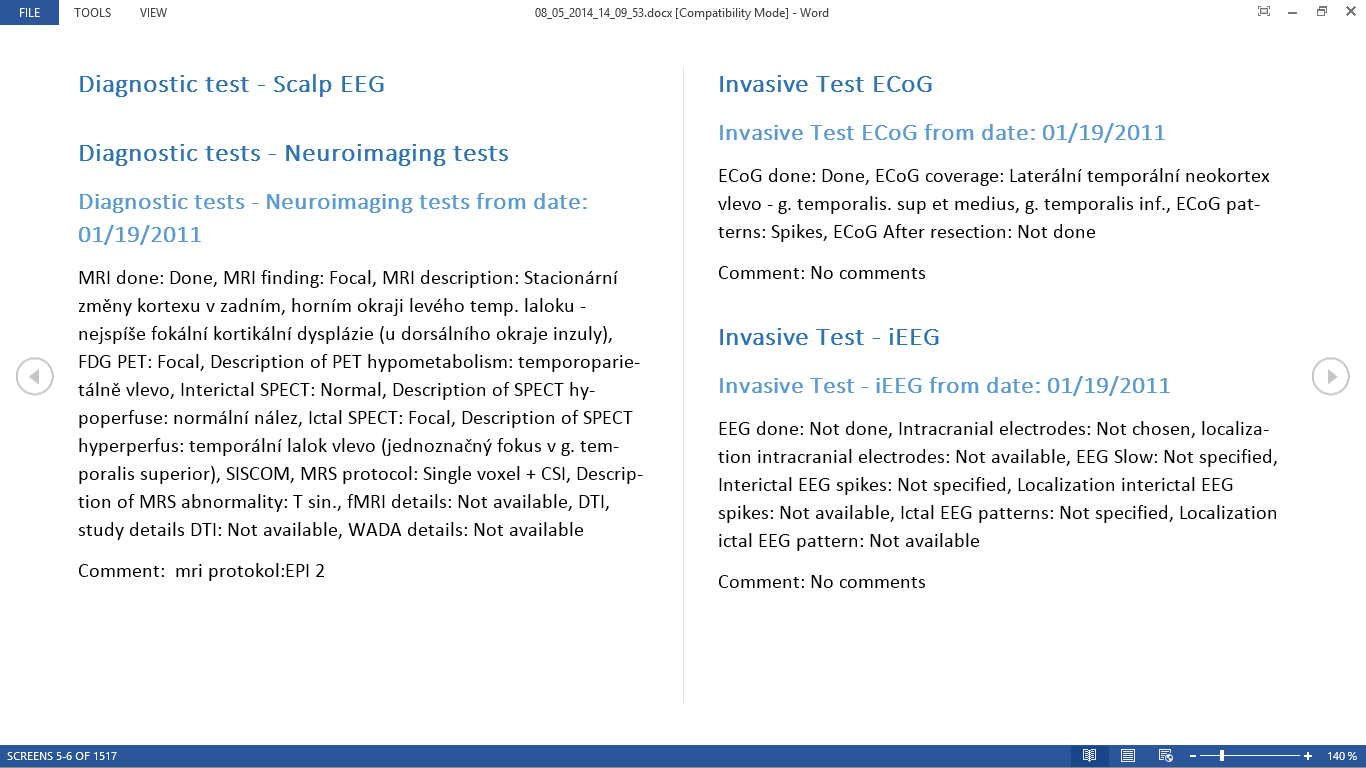
\includegraphics[width=1\textwidth]{images/docxExport_2.png}
 	\caption{Screenshot of an export of all patients to docx}
 	\label{fig:docxExport_2}
\end{figure}

\begin{figure}
	\centering
 	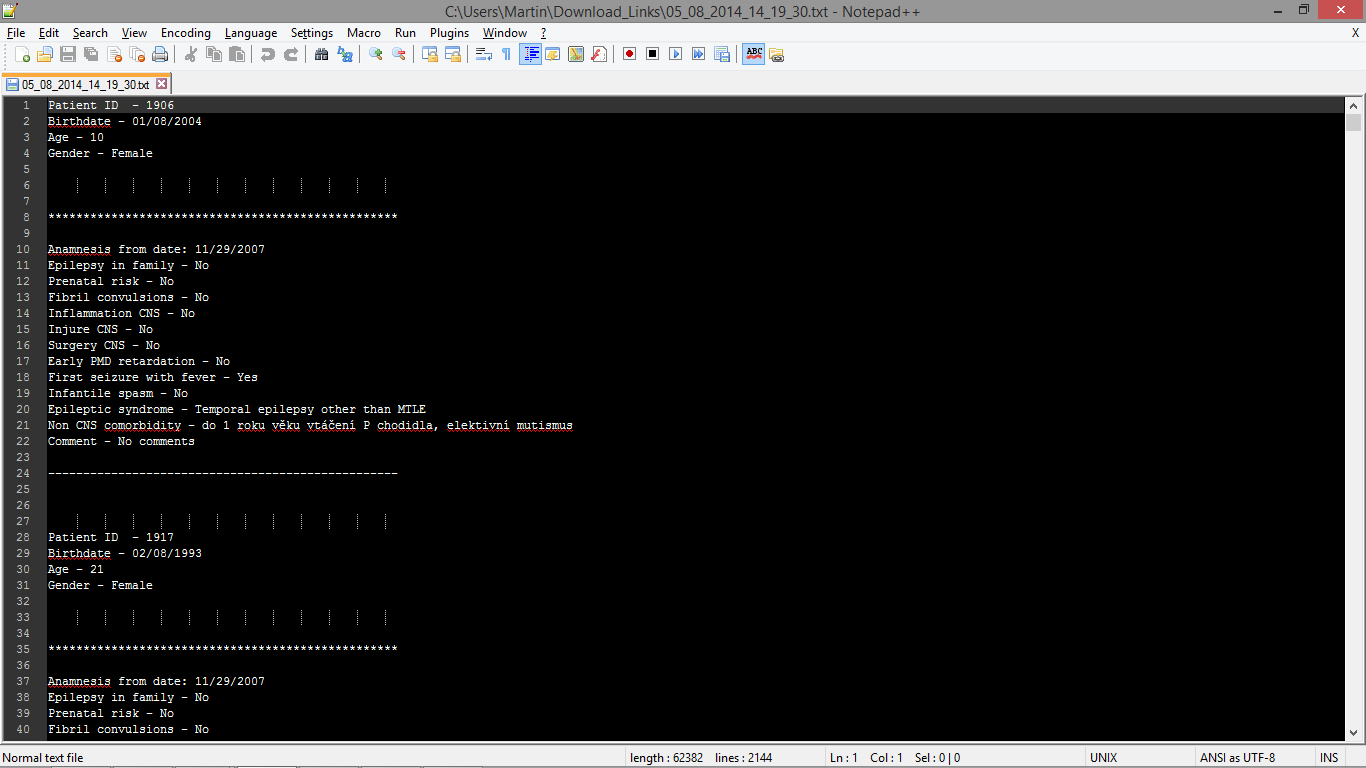
\includegraphics[width=1\textwidth]{images/txtExport.png}
 	\caption{Screenshot of an export of all female patients to txt}
 	\label{fig:txtExport}
\end{figure}

\begin{figure}
	\centering
 	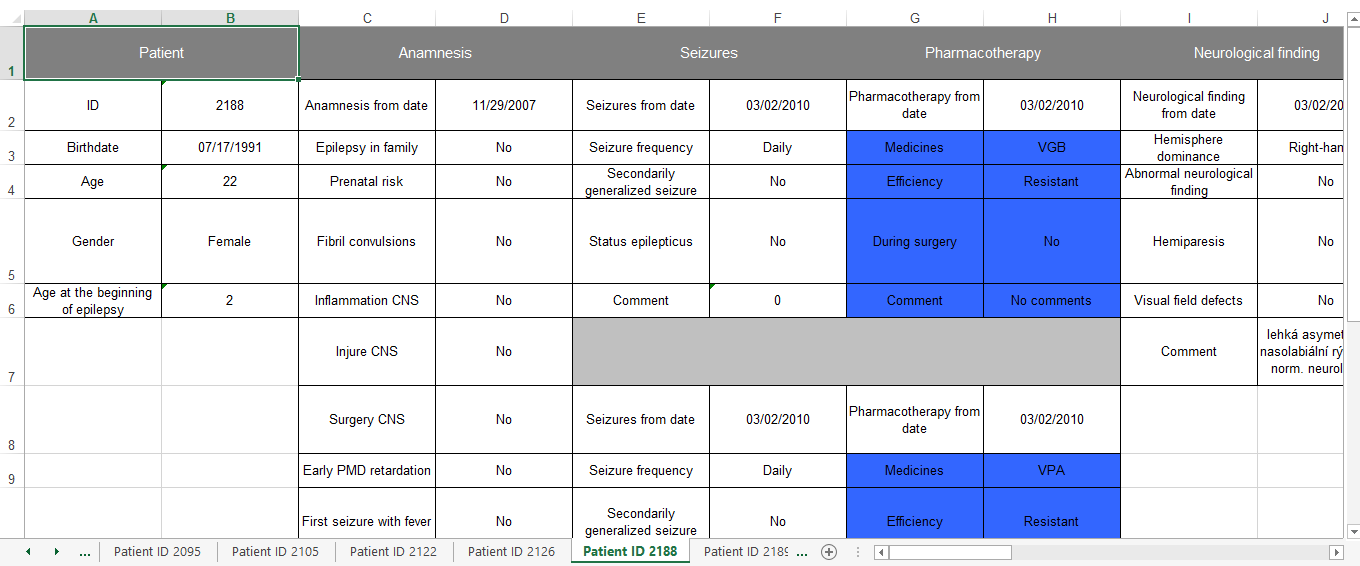
\includegraphics[width=1\textwidth]{images/xlsExport_1.png}
 	\caption{Screenshot of an export of all patients older then 5 years to xls}
 	\label{fig:xlsExport_1}
\end{figure}


\begin{figure}
	\centering
 	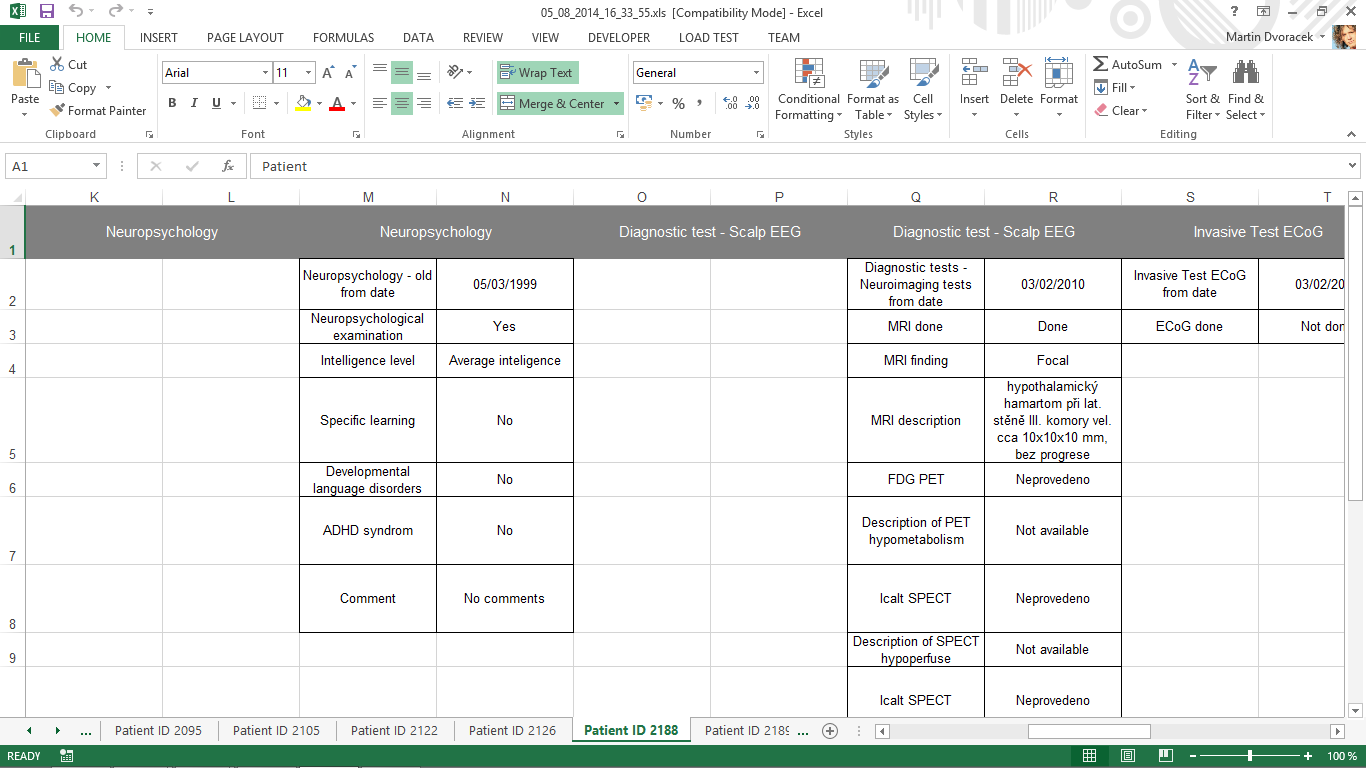
\includegraphics[width=1\textwidth]{images/xlsExport_2.png}
 	\caption{Screenshot of an export of all patients older then 5 years to xls}
 	\label{fig:xlsExport_2}
\end{figure}

\begin{figure}
	\centering
 	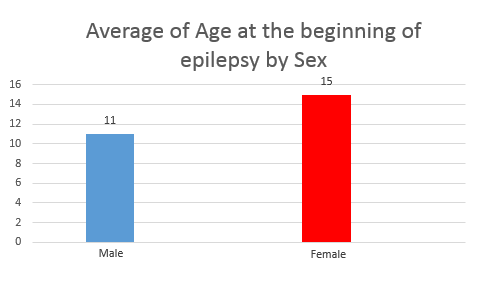
\includegraphics[width=1\textwidth]{images/chart.png}
 	\caption{Example of an analysis from exported data}
 	\label{fig:chart}
\end{figure}
\begin{conclusion}
I've created a tool that greatly extends the possibilities that GENEPI IS could provide to doctors and researchers who use it. Without the reporting module GENEPI IS would be only a tool to store and look up informations about patients. But now it becomes a tool, that can provide to users structured and customized reports. Those reports may be used as a source of important information about the patient's state of health and about the process of his treatment through surgery as well as a source of data for analysis and research.

Thanks to the possibility to customize exports the doctors can select to export only that data which is important for a given medical intervention. As it is expected that the set of requested information to given interventions will not change frequently, the doctors can also use the feature of the module to configure the export once, then save the configuration and then just load it anytime they would need it, without any need of further configuration.

Another possibility of using the reporting module are analyses made by researchers. Researchers shouldn't usually be allowed to see sensitive data about patients. Thus the feature of automatical anonymazation of the patient's data comes in handy. Also a possibility to export an unlimited numer of patients during one export to one file is useful, because researchers need a larger amount of data to make any analysis. Exporting every single patient to separate files one by one, would be a really user-unfriendly solution. It is also expected, that researchers will use different formats than doctors. Whereas doctors are expected to use mostly docx or pdf format, researchers will probably use xls, csv or txt. These formats can be easily parsed and processed to other software for further analysis.

For all these reasons it is now possible to execute export to 14 sundry formats. Those are 5 basic formats, 5 more in anonymized variant. Docx and pdf export can be also formated to tables. With the anonymized variant we get 4 more formats. This solution should be sufficient to meet the needs of any user of GENEPI IS.

To sum up, all goals stated in the beginning of this thesis were satisfied. Moreover, I've added some features that may ease the work with the reporting module, such as generic configurations or more types of formatting when exporting to docx and pdf.

I must say I'm really satisfied with the software I've created on the basis of the requests of the doctors from the Faculty Hospital Motol in Prague. I belive that it will serve doctors and researchers well and make their work and research much easier. This all should lead to an improvement of the treatment of patients with epilepsy.

I'm proud that result of my bachelor's thesis will be deployed in the biggest hospital in the Czech Republic and will be used there to help real patients. I also believe that that my work will have its share on helping all mankind to understand such an insidious disease such an epilepsy is and maybe even to save somebody's life.

\end{conclusion}

\bibliographystyle{iso690}
\bibliography{mybibliographyfile}

\appendix

\chapter{Acronyms}
% \printglossaries
\begin{description}
	\item[API] Application Programming Interface
	\item[AS] Application Server
	\item[BO] Business Object
	\item[CI] Continuous Integration
	\item[DAO] Data Access Object
	\item[GUI] Graphical User Interface
	\item[HQL] Hibernate Query Language
	\item[IS] Information System
	\item[JDBC] Java Database Connectivity
	\item[JSP] JavaServer Page
	\item[MD] Manday
	\item[MVC] Model View Controller
	\item[XML] Extensible Markup Language
\end{description}

\chapter{Contents of enclosed CD}
To my bachelor's thesis I enclose a CD which contains all the important data, needed to depoloy GENEPI IS. It also contains source codes of GENEPI IS and the libraries that it uses. In the installPackage directory is also an enclosed a model for MySQL Workbench, where the reader may see the structure of the database. In the same folder you can also find a directory with migration scripts. These are important when migrating from the information system that was previously used in the Faculty Hospital Motol to GENEPI IS. Migration scripts allow you to copy data from the previously used database to the databse that is being used by the GENEPI IS. Thanks to this, the reader should be able to administrate or even modify GENEPI IS without any larger problems.

The next important directory is the directory with samples of exported data. This folder contains 14 files with all possible formats of exported data - pdf, docx, xls, csv, txt - all of these formates in both anonymized and unanonymized variants (sensitive data were changed) and both printed as a plain text and formated to a table for pdf and docx as well.

The reader will also find a useful directory that contains deployment packages of the results of the previously mentioned projects from the subjects BI-SP1 and BI-SP2. The documentation to these doesn't differ from the documentation for the GENEPI IS.

I would also recommend you become familiar with the content of the directory documentation, where you will find user and admin documentation for GENEPI IS.

Additional content of the enclosed CD is the text directory, that contains this theis in a pdf format.

\begin{figure}
	\dirtree{%		
.1 documentation\DTcomment{the directory of the GENEPI IS documentation}.		
		.1 installPackage\DTcomment{the directory of install package of the current version}.
		.1 previousVersions\DTcomment{the direcotry of the results of BI-SP1 and BI-SP2}.
		.1 sampleData\DTcomment{the directory that contains samples of exported data}.
		.1 source\DTcomment{the directory of source codes of the GENEPI IS and this thesis}.
		.2 impl\DTcomment{the directory of source codes of the GENEPI IS}.
		.3 images \DTcomment{the directory of images used in the thesis}.
		.3 thesis.ps\DTcomment{the thesis text in PS format}.		
		.3 Backend\DTcomment{the directory of a maven project}.
		.4 src\DTcomment{the directory of GENEPI IS source codes}.
		.5 main.
		.6 java.
		.7 cz.
		.8 cvut.
		.9 fit.
		.10 GENEPI\DTcomment{the directory of java classes}.
		.6 resources\DTcomment{the directory configuration files}.
		.6 webapp.
		.7 resources\DTcomment{the directory of librarires for front end}.
		.8 WEB-IF.
		.9 spring\DTcomment{the directory for spring context file}.
		.9 tags\DTcomment{the directory of templates for jsp pages}.
		.9 views\DTcomment{the directory of jsp pages}.
		.5 test\DTcomment{the directory of source codes of unit tests }.
		.2 thesis\DTcomment{the directory of source codes of this thesis}.
		.1 text\DTcomment{the thesis text directory}.
		.2 BachelorsThesis.pdf\DTcomment{the thesis text in PDF format}.
		.1 readme.txt\DTcomment{the file with CD contents description}.
	}
\end{figure}

\end{document}
